\chapter{Motivation}
\label{motiv}
In the institute of reliable Embedded Systems and Communication Electronics
(ivESK) is a project named \embtls which has the goal to use the TLS protocol
(see chapter \ref{tls_proto}) in embedded systems.

\begin{figure}[!ht]
\centering
%\frame{
% trim: left, bottom, right, up
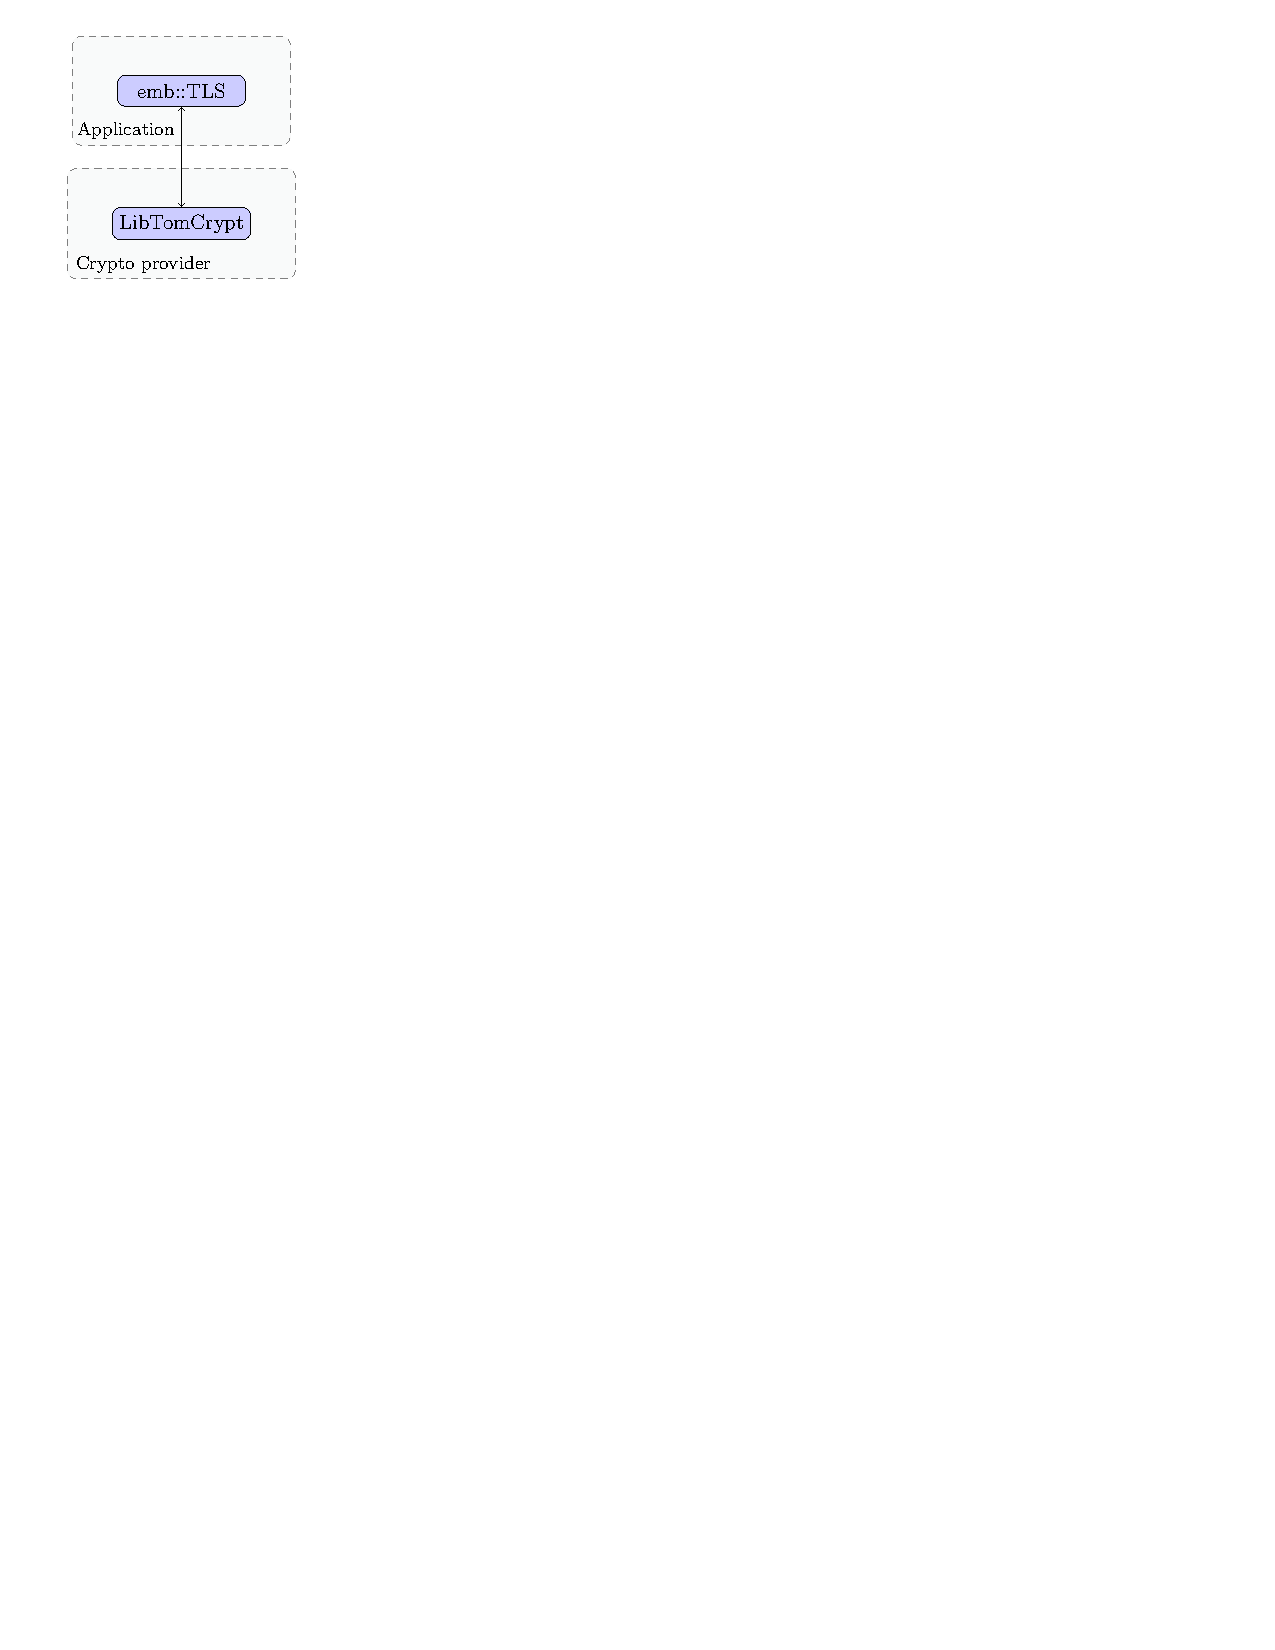
\includegraphics[trim=0cm 23.25cm 15cm 0cm,
height=6.5cm]{figures/intro_embtls.pdf}
\caption{\embtls's project}
\label{fig:motiv_embtls}
%}

\end{figure}
For this, a cryptographic provider (\tomcrypt) is used for the part of
cryptographic calculation needed for the application.
This cryptographic provider is an open-source cryptography software
library.
Problems with this implementation is that only \tomcrypt is
supported as cryptographic providers, meaning that no other libraries can be used
without changing the complete implementation for \embtls.

\begin{figure}[!ht]
\centering
%\frame{
% trim: left, bottom, right, up
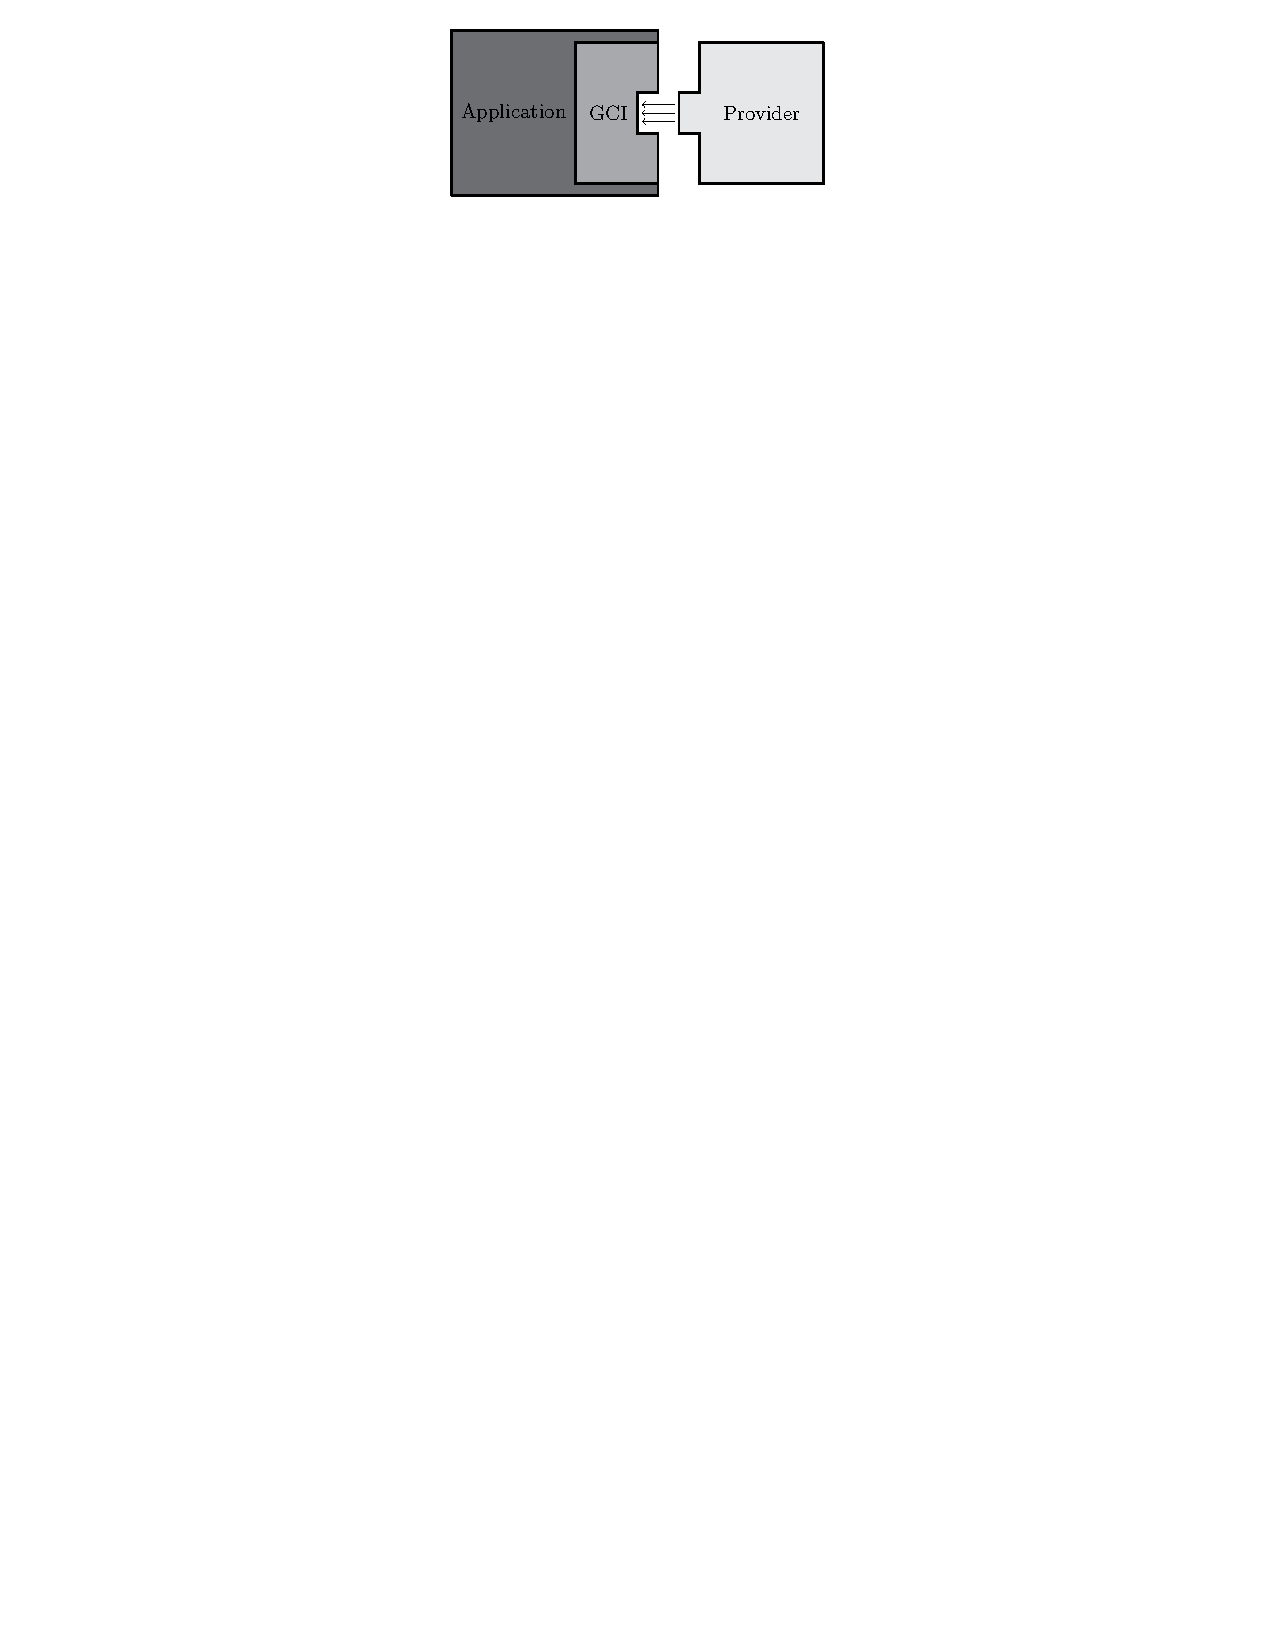
\includegraphics[trim=6cm 24.5cm 2cm 0cm, height=6cm]{figures/intro_gci.pdf}
\caption{Goal of the new implementation}
\label{fig:motiv_gci}
%}
\end{figure}
The goal of the project is therefore to create an interface, a Generic
Cryptographic Interface (GCI), to have a base of the existing cryptography
services and to have the possibility to easily change the providers only by
changing some lines in the interface, instead of the complete
implementation.\newline
Through to this new interface other new cryptographic algorithms may be
easier to add in the interface and to use for the application.\newline
As shown on the figure \ref{fig:motiv_gci}, the interface is implemented in the
application and nothing has to be changed.
The requirements for this Generic Cryptographic Interface (GCI) are listed
below:
\begin{enumerate}
  \item No hidden states shall be used in the interface, meaning that the
  behavior of the cryptographic algorithm functions should only be affected by
  the input parameters.
  All parameters written in input of the function will be used for the
  cryptographic algorithm and nothing else.
  \item Different cryptographic providers may be used for the cryptographic
  calculation. \newline
  That could be open-source cryptographic software libraries or hardware-based cryptographic modules.
  \item With the old version of the implementation (figure
  \ref{fig:motiv_embtls}), the application and the provider interact, meaning
  that when the provider needs informations from the application, this one just send them and
  vice-versa.
  With this new implementation (figure \ref{fig:motiv_gci}) the interface break
  this interaction. To always have this interaction, the interface shall receive
  the information from the application and the provider. These informations
  shall be easily used by both (application and provider) when needed.
\end{enumerate}
 